\documentclass[journal]{IEEEtran}

\usepackage[T1]{fontenc}
\usepackage{cite}
\usepackage{amsmath,amssymb,amsfonts}
\usepackage{graphicx}
\usepackage{textcomp}
\usepackage{booktabs}
\usepackage{tabularx}
\usepackage{multirow}
\usepackage{array}
\usepackage{algorithm}
\usepackage{algpseudocode}
\usepackage{url}
\usepackage{balance}
\usepackage{placeins}

\hyphenation{know-ledge trans-for-ma-tion read-i-ness gra-di-ent boost-ing}

\begin{document}

\title{A Knowledge-Based AI Decision-Support Model for Predicting Digital Transformation Readiness From Enterprise Innovation Data}

\author{Vineeth~Kumar~Samba%
\thanks{Manuscript received 23 October 2026.}%
\thanks{V. K. Samba is with SoftTechers LLC, Charlotte, NC 28262 USA
(e-mail: vineethkumarsamba@gmail.com).}}

\markboth{IEEE Transactions on Knowledge and Data Engineering,~Vol.~XX, No.~X, 2026}%
{Samba: Knowledge-Based Decision Support for Digital Transformation Readiness}

\maketitle

\begin{abstract}
Predicting whether a firm is ready for digital transformation is a small-data problem: few organizations have labeled readiness outcomes, yet experts hold well-developed maturity models. This paper presents KB-DSS, a knowledge-based decision-support model that predicts three-level digital transformation readiness (DTR) from 12 enterprise innovation indicators, firm size, and sector. A knowledge layer encodes five expert pillars (data, technology, organization, governance, and innovation), six signed fuzzy IF--THEN rules, and a zero-training expert index. These knowledge features are appended to the raw inputs of a gradient-boosting learner, and every prediction is returned with a rule trace, the firm's two weakest pillars, and recommended actions. The central novelty is a knowledge-fidelity protocol that degrades the knowledge layer in controlled steps (fidelity \(\varphi\) from 1.0 to 0.0) and measures the value of knowledge as a function of both knowledge quality and training-set size. On a reproducible benchmark of 2000 synthetic firms, correct knowledge raised gradient-boosting Macro-F1 by 0.075 (95\% CI 0.059 to 0.091) with 60 training firms and by 0.022 (0.015 to 0.028) with 1500. The gain shrank as fidelity fell, and fully misspecified knowledge gave no gain beyond 60 firms. Under 15\% training-label noise, KB-DSS held Macro-F1 0.791 while plain boosting fell to 0.766. Under corrected \(5\times 3\) cross-validation at 1600 training firms, however, KB-DSS (0.803) did not differ significantly from plain boosting (\(+0.013\), 95\% CI \(-0.004\) to \(+0.031\)) or from logistic regression (0.810). The results therefore support a bounded claim: expert knowledge is most valuable when it is correct, data are scarce or labels are noisy, and its value can be measured before deployment.
\end{abstract}

\begin{IEEEkeywords}
Decision support systems, digital transformation, explainable artificial intelligence, fuzzy systems, gradient boosting, informed machine learning, knowledge-based systems, small-sample learning.
\end{IEEEkeywords}

\section{Introduction}

Digital transformation changes how firms create value through data, platforms, and new organizational routines~\cite{vial2019}. Before committing capital, managers and entrepreneurs need to know whether their data, technology, people, governance, and innovation capability are ready. Practice answers this with digital maturity models, but a review of 22 such models found that their dimensions differ widely and that culture and transformational capability are often missing~\cite{teichert2019}; a 2026 review reaches a similar conclusion for the newer generation of models~\cite{stef2026}. Adoption research explains readiness through the technology--organization--environment (TOE) framework~\cite{tornatzky1990}. A systematic review of 106 studies of AI adoption in small and medium enterprises organizes the field along these lines~\cite{schwaeke2025}. These approaches are transparent but explanatory: they rank firms with expert-set weights and do not learn from outcome data.

Two computational lines address readiness. Knowledge-driven systems encode expert judgment directly: fuzzy logic and the analytic hierarchy process have been used to assess digitalization barriers in 4531 SMEs~\cite{restrepo2024}, and a knowledge-based expert system evaluated digital supply-chain readiness~\cite{khan2021}. Data-driven systems learn from firm records: ensemble learners such as XGBoost and LightGBM predicted digital transformation of Chinese listed firms better than linear regression~\cite{chen2024}. The first line cannot correct its own weights; the second needs many labeled firms and returns a class without a reason a manager can act on~\cite{barredo2020}.

Informed machine learning proposes to integrate prior knowledge into the learning pipeline~\cite{vonrueden2023}, and recent work combines data- and knowledge-driven rules for classification~\cite{geng2024} or uses large language models to generate rule features for few-shot tabular learning~\cite{han2024}. One question is rarely measured directly, however: how much is the knowledge worth, and when? Expert models are never fully correct, and a knowledge layer that is wrong may add noise rather than signal. A decision-support system should therefore report not only its accuracy but also how its gain depends on the quality of the knowledge and on the amount of data available.

This paper asks two research questions. RQ1: does a fuzzy-rule knowledge layer improve readiness prediction by a gradient-boosting learner, and under which data conditions? RQ2: how does that improvement change as the knowledge becomes less correct? The contribution is threefold: (i)~KB-DSS, a compact knowledge layer of five pillars, six signed fuzzy rules, and an expert index for DTR, coupled to a hybrid learner that returns rule-trace explanations; (ii)~a knowledge-fidelity protocol that degrades the knowledge layer in controlled steps and maps its value across fidelity and training-set size; and (iii)~a reproducible benchmark with five baselines, component ablation, label-noise stress tests, and corrected resampled statistics, released as a single script that also runs on real data.

\section{Proposed KB-DSS Framework}

KB-DSS has four stages (Fig.~\ref{fig:framework}): enterprise data, a knowledge layer, a hybrid learner, and a decision-support output.

\begin{figure*}[!t]
\centering
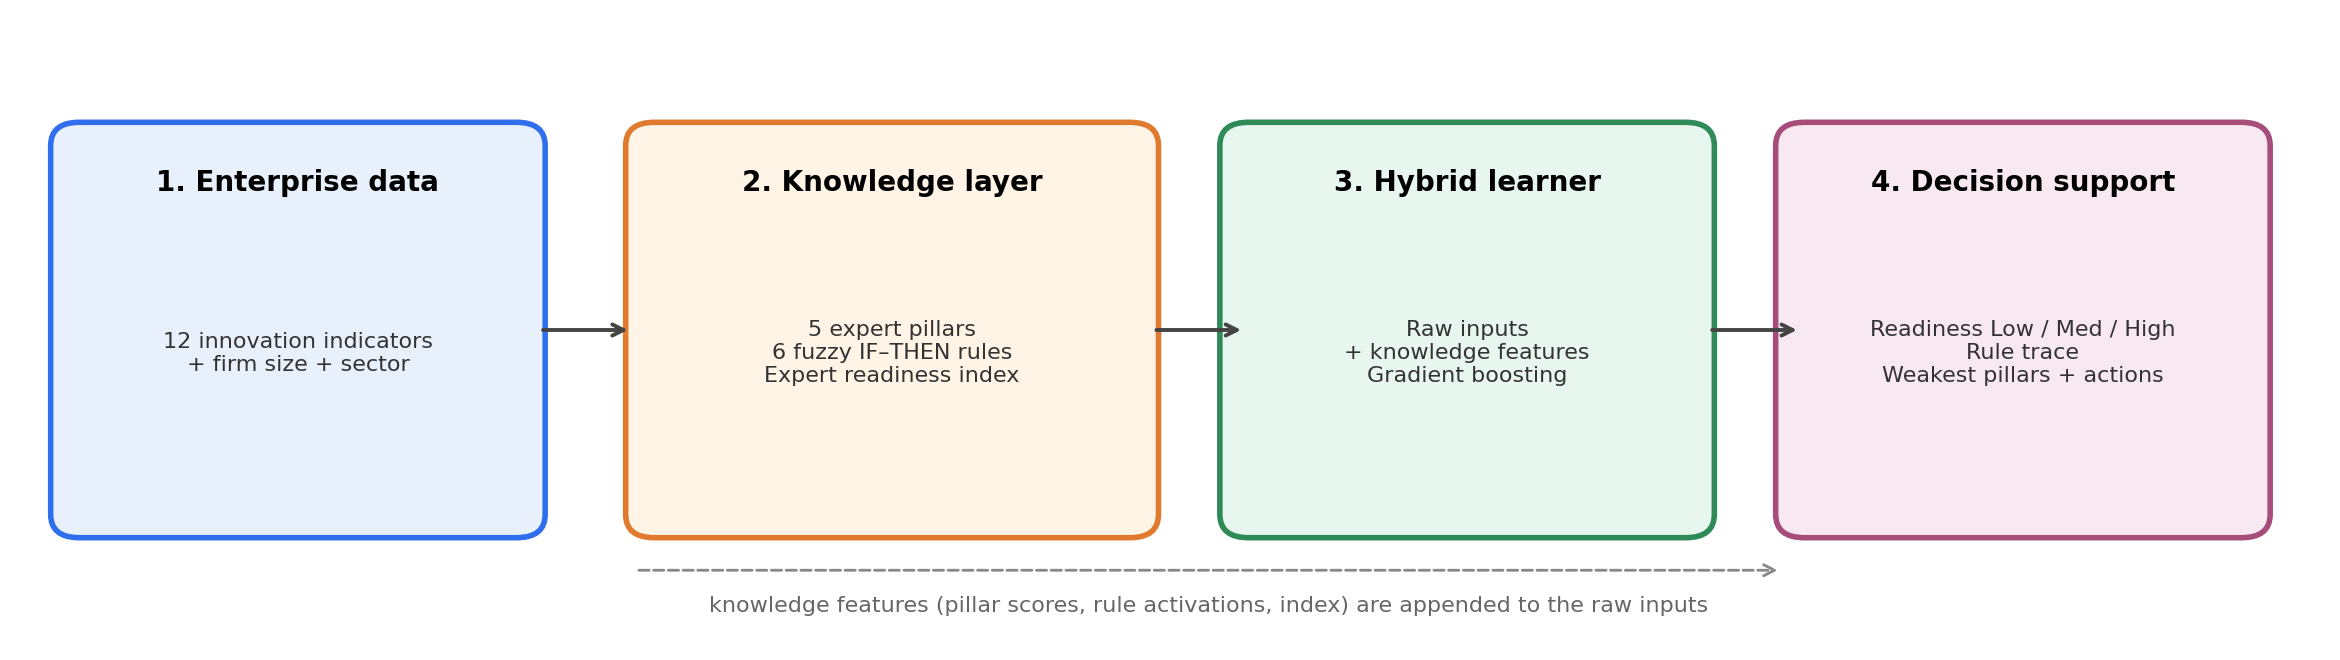
\includegraphics[width=0.95\textwidth]{figures/fig1.png}
\caption{The KB-DSS framework. The knowledge layer turns the 12 indicators into 5 pillar scores, 6 fuzzy rule activations, and 1 expert index; these 12 knowledge features are appended to the 13 raw inputs and sector before learning.}
\label{fig:framework}
\end{figure*}

\subsection{Firm Representation}

A firm is described by \(\mathbf{x}=(x_1,\ldots,x_{12})\in[0,1]^{12}\): data maturity, analytics capability, AI adoption, cloud adoption, data governance, leadership commitment, digital skills, R\&D intensity, innovation output, entrepreneurial orientation, legacy debt, and regulatory intensity, plus a standardized log firm size and one of five sectors. The target is readiness \(y\in\{\mathrm{Low},\mathrm{Medium},\mathrm{High}\}\).

\subsection{Knowledge Layer}

Five expert pillars summarize the indicators, following the dimensions shared by maturity models~\cite{teichert2019} and the TOE framework~\cite{tornatzky1990}. Each pillar \(k\) has a set of indicators \(J_k\) with signed expert weights \(w_{kj}\), and its score is a weighted mean in \([0,1]\):
\begin{equation}
P_k(\mathbf{x})
=
\frac{\sum_{j\in J_k}|w_{kj}|\,\tilde{x}_j}{\sum_{j\in J_k}|w_{kj}|},
\qquad
\tilde{x}_j
=
\begin{cases}
x_j, & w_{kj}>0,\\
1-x_j, & w_{kj}<0.
\end{cases}
\label{eq:pillar}
\end{equation}
The pillars are Data (data maturity 0.5, analytics capability 0.5), Technology (AI adoption 0.35, cloud adoption 0.35, legacy debt \(-0.30\)), Organization (leadership commitment 0.5, digital skills 0.5), Governance (data governance 1.0), and Innovation (R\&D intensity 0.30, innovation output 0.35, entrepreneurial orientation 0.35).

Six signed fuzzy IF--THEN rules capture interactions that a weighted sum cannot. Each rule \(r\) has an antecedent of literals \(\ell\) (an indicator or its complement) combined with the minimum \(t\)-norm as fuzzy AND~\cite{zadeh1965}, and a sign \(s_r\in\{+1,-1\}\) for its expert effect on readiness:
\begin{equation}
\mu_r(\mathbf{x})
=
\min_{\ell\in A_r}\ell(\mathbf{x}),
\qquad
\ell(\mathbf{x})\in\{x_j,\;1-x_j\}.
\label{eq:rule}
\end{equation}
The rule base \(R=\{R_1,\ldots,R_6\}\) is:
\begin{enumerate}
\item \(R_1\), data--AI synergy (\(+\)): data maturity AND AI adoption.
\item \(R_2\), governance gap (\(-\)): AI adoption AND \((1-\text{data governance})\) AND regulatory intensity.
\item \(R_3\), legacy barrier (\(-\)): legacy debt AND \((1-\text{cloud adoption})\).
\item \(R_4\), sponsor capability (\(+\)): leadership commitment AND digital skills.
\item \(R_5\), innovation engine (\(+\)): R\&D intensity AND entrepreneurial orientation.
\item \(R_6\), analytics without a base (\(-\)): analytics capability AND \((1-\text{data maturity})\).
\end{enumerate}
The expert readiness index combines pillars and rules:
\begin{equation}
E(\mathbf{x})
=
\sum_{k=1}^{5}\omega_k P_k(\mathbf{x})
+
\frac{\lambda}{6}\sum_{r=1}^{6}s_r\,\mu_r(\mathbf{x}),
\label{eq:index}
\end{equation}
with \(\boldsymbol{\omega}=(0.25,0.20,0.25,0.15,0.15)\) and \(\lambda=0.35\). Used alone, \(E(\mathbf{x})\) is a zero-training classifier: the two class thresholds are set at the quantiles of \(E\) on the training firms that match the training class priors. The weights were set by the author from maturity-model and TOE logic before any experiment and were not tuned on the data.

\subsection{Hybrid Learner}

The knowledge map \(\kappa(\mathbf{x})=[P_1,\ldots,P_5,\mu_1,\ldots,\mu_6,E]\) produces 12 knowledge features. KB-DSS learns a classifier on the raw inputs joined with them:
\begin{equation}
\hat{y}
=
\arg\max_{c}\,
f_c\bigl(\mathbf{x}\oplus\kappa(\mathbf{x})\bigr),
\label{eq:hybrid}
\end{equation}
where \(f\) is a histogram gradient-boosting classifier~\cite{friedman2001,pedregosa2011} with 150 iterations, learning rate 0.06, maximum depth 3, and L2 penalty 1.0, and \(\oplus\) denotes concatenation. Gradient boosting was chosen because tree ensembles remain the strongest general-purpose learners for tabular data~\cite{grinsztajn2022}. Because \(\kappa\) is fixed and deterministic, the knowledge is injected as features: the learner may use, reweight, or ignore each expert signal.

\subsection{Explanation and Recommendation}

For any firm, KB-DSS returns the predicted class and probabilities, the two lowest pillar scores, every rule with activation \(\mu_r>0.4\) and its sign, and one recommended action for each weak pillar and each fired negative rule. Explanations come from the additive structure of~\eqref{eq:pillar}--\eqref{eq:index}, not from a post-hoc approximation of the learner~\cite{barredo2020}. Algorithm~\ref{alg:kbdss} summarizes the procedure.

\begin{algorithm}[t]
\caption{KB-DSS Readiness Prediction and Explanation}
\label{alg:kbdss}
\begin{algorithmic}[1]
\Require Training firms \(\{(\mathbf{x}_i,y_i)\}\), weights \(w\), rules \(R\), \((\boldsymbol{\omega},\lambda)\)
\Ensure Class, probabilities, rule trace, actions
\For{each firm \(\mathbf{x}_i\)}
    \State compute pillar scores \(P_k(\mathbf{x}_i)\) by~\eqref{eq:pillar}
    \State compute rule activations \(\mu_r(\mathbf{x}_i)\) by~\eqref{eq:rule}
    \State compute expert index \(E(\mathbf{x}_i)\) by~\eqref{eq:index}
    \State form the joint vector \(\mathbf{x}_i\oplus\kappa(\mathbf{x}_i)\)
\EndFor
\State fit gradient boosting \(f\) on \(\{(\mathbf{x}_i\oplus\kappa(\mathbf{x}_i),y_i)\}\)
\State for a new firm \(\mathbf{x}\): predict class and probabilities by~\eqref{eq:hybrid}
\State report the two weakest pillars and every rule with \(\mu_r(\mathbf{x})>0.4\)
\State emit one action per weak pillar and per fired negative rule
\end{algorithmic}
\end{algorithm}

\section{Experimental Design}

\subsection{Benchmark}

No public dataset links enterprise innovation indicators to a labeled readiness level, so the study uses a reproducible synthetic benchmark of 2000 firms (seed 42). Each indicator mixes a firm-specific \(\mathrm{Beta}(2,2)\) draw with a shared \(\mathrm{Beta}(2.2,2.2)\) ``digital culture'' factor, so indicators are positively correlated as in survey data. Legacy debt falls with cloud adoption, regulatory intensity is higher in finance and healthcare, and data governance rises with regulation. A latent readiness score is a weighted sum of the 12 indicators with weights that differ from the expert weights, four interaction terms that share the form of rules \(R_1\), \(R_2\), \(R_3\), and \(R_5\), a cloud-by-size interaction and sector effects that no rule encodes, and Gaussian noise (SD 0.55). The 30th and 70th percentiles of the latent score define Low, Medium, and High readiness (600, 800, and 600 firms). Rules \(R_4\) and \(R_6\) have no counterpart in the generator. The knowledge layer is therefore a partial and imperfect model of the data, and the benchmark is designed so that no method can recover it exactly.

\subsection{Baselines and Metrics}

Six models were compared: the zero-training expert index~\eqref{eq:index}; logistic regression, random forest~\cite{breiman2001}, and plain gradient boosting on raw inputs; KB-LR, a logistic regression on raw plus knowledge features; and KB-DSS. KB-DSS was fixed as the proposed model in the code before any result was inspected. The metrics are accuracy, Macro-F1 (primary), and quadratic weighted kappa (QWK)~\cite{cohen1968}, which credits near misses on the ordinal readiness scale.

\subsection{Knowledge-Fidelity Protocol}

To measure what the knowledge is worth, the knowledge layer is degraded in controlled steps. Fidelity \(\varphi\in\{1.0,0.75,0.50,0.25,0.0\}\) is the share of the 12 indicators that the knowledge layer reads correctly. For \(\varphi<1\), a random subset of \(\mathrm{round}((1-\varphi)\cdot 12)\) indicators is cyclically swapped before~\eqref{eq:pillar}--\eqref{eq:index} are evaluated:
\begin{equation}
\kappa_{\varphi}(\mathbf{x})=\kappa(\Pi_{\varphi}\,\mathbf{x}),
\quad
\Pi_{1.0}=I,
\label{eq:fidelity}
\end{equation}
where \(\Pi_{0.0}\) moves all 12 indicators.
The learner always sees the correct raw inputs; only the expert layer is wrong. At \(\varphi=0\) the pillars and rules still aggregate real indicators, but in the wrong roles. This separates the value of correct domain structure from the generic value of adding aggregate features.

\subsection{Evaluation Protocol and Statistics}

The main comparison (Table~\ref{tab:models}) and the ablation (Table~\ref{tab:ablation}) use 5-fold stratified cross-validation repeated 3 times (15 folds, 1600 training firms each). Because training sets overlap across folds, naive paired tests overstate significance~\cite{demsar2006}. Differences in Macro-F1 are therefore tested with the Nadeau--Bengio corrected resampled \(t\)-test~\cite{nadeau2003}:
\begin{equation}
t
=
\frac{\bar{d}}{\sqrt{\bigl(\tfrac{1}{J}+\tfrac{n_{\mathrm{test}}}{n_{\mathrm{train}}}\bigr)s_d^2}},
\qquad
J=15,
\quad
\frac{n_{\mathrm{test}}}{n_{\mathrm{train}}}=\frac{1}{4},
\label{eq:nadeau}
\end{equation}
where \(\bar{d}\) and \(s_d^2\) are the mean and variance of the per-fold differences, with \(J-1\) degrees of freedom. The learning-curve and fidelity sweep (Fig.~\ref{fig:results}) uses 12 random stratified splits, each with a 400-firm hold-out and training subsets of 60 to 1500 firms drawn from the remaining 1600; each split draws its own fidelity permutations. In total the sweep fits 648 models. Permutation importance (20 repeats) is computed on one 400-firm hold-out. The full study runs in about five minutes on a laptop CPU, and a self-test checks the invariants of the knowledge layer before every run.

\section{Results and Discussion}

\subsection{Performance With Ample Data}

With 1600 training firms, KB-DSS reached Macro-F1 0.803 and QWK 0.827, above plain gradient boosting (0.790), the random forest (0.790), and the expert index (0.782), and below logistic regression (0.810) and KB-LR (0.811) (Table~\ref{tab:models}). None of these differences is significant under the corrected test. The gain over plain boosting is \(+0.013\) (95\% CI \(-0.004\) to \(+0.031\), \(p=0.130\)). A naive paired Wilcoxon test on the same 15 folds gives \(p=0.005\) for this comparison, which shows how far overlapping folds can overstate significance~\cite{nadeau2003,demsar2006}. Logistic regression is competitive because the latent score is mostly additive; adding knowledge features to it changes Macro-F1 by only 0.001.

\begin{table*}[!t]
\caption{Model Comparison Under Repeated Stratified Cross-Validation (2000 Firms, 1600 Training Firms Per Fold)}
\label{tab:models}
\centering
\setlength{\tabcolsep}{4pt}
\scriptsize
\begin{tabular*}{\textwidth}{@{\extracolsep{\fill}}lccccc}
\toprule
Model & Accuracy & Macro-F1 & QWK & Gain vs row [95\% CI] & \(p\) \\
\midrule
Expert index (zero training)
  & \(0.776\pm0.018\) & \(0.782\pm0.018\) & \(0.813\pm0.016\) & \(+0.021\) [\(-0.002\), \(+0.044\)] & 0.074 \\
Logistic regression
  & \(0.805\pm0.022\) & \(0.810\pm0.021\) & \(0.835\pm0.019\) & \(-0.007\) [\(-0.024\), \(+0.009\)] & 0.350 \\
Random forest
  & \(0.784\pm0.020\) & \(0.790\pm0.020\) & \(0.812\pm0.018\) & \(+0.013\) [\(-0.004\), \(+0.030\)] & 0.134 \\
Gradient boosting
  & \(0.784\pm0.022\) & \(0.790\pm0.021\) & \(0.816\pm0.019\) & \(+0.013\) [\(-0.004\), \(+0.031\)] & 0.130 \\
KB-LR (logistic + knowledge)
  & \(0.806\pm0.023\) & \(0.811\pm0.022\) & \(0.836\pm0.019\) & \(-0.008\) [\(-0.026\), \(+0.010\)] & 0.358 \\
KB-DSS (proposed)
  & \(0.797\pm0.022\) & \(0.803\pm0.022\) & \(0.827\pm0.017\) & --- & --- \\
\bottomrule
\end{tabular*}
\vspace{2pt}

{\raggedright\scriptsize 5-fold CV repeated 3 times (15 folds). Values are mean \(\pm\) SD. Gain is KB-DSS minus the row model in Macro-F1, with a Nadeau--Bengio corrected 95\% CI and \(p\)-value~\cite{nadeau2003}.\par}
\end{table*}

\subsection{Component Ablation and Stress Tests}

Each knowledge component raised the Macro-F1 of gradient boosting (Table~\ref{tab:ablation}): pillars by 0.004, rules by 0.010, and the expert index by 0.020, the only interval that excludes zero. The full layer added 0.013. The index-only variant was better than the full layer in this run; it was found after the fact, so it is reported as an observation and was not used to choose the proposed model. Two stress tests isolate what the knowledge contributes. When all 12 indicators were permuted before the knowledge layer read them, the gain vanished (\(+0.000\), 95\% CI \(-0.011\) to \(+0.011\)). The benefit therefore comes from correct expert structure, not from extra features as such. When 15\% of training labels were corrupted, plain boosting lost 0.024 Macro-F1 (95\% CI \(-0.041\) to \(-0.007\)), while KB-DSS held 0.791, essentially the clean baseline (\(+0.002\)). Expert features act as a label-independent anchor that noisy labels cannot shift.

\begin{table*}[!t]
\caption{Component Ablation and Stress Tests for Gradient Boosting}
\label{tab:ablation}
\centering
\setlength{\tabcolsep}{6pt}
\scriptsize
\begin{tabular*}{\textwidth}{@{\extracolsep{\fill}}lccc}
\toprule
Variant & Macro-F1 & QWK & \(\Delta\) Macro-F1 vs raw [95\% CI] \\
\midrule
Raw features only (no knowledge)
  & \(0.790\pm0.021\) & \(0.816\pm0.019\) & --- \\
\(+\) pillar scores only
  & \(0.794\pm0.019\) & \(0.820\pm0.016\) & \(+0.004\) [\(-0.012\), \(+0.020\)] \\
\(+\) fuzzy rules only
  & \(0.800\pm0.020\) & \(0.825\pm0.017\) & \(+0.010\) [\(-0.003\), \(+0.024\)] \\
\(+\) expert index only
  & \(0.810\pm0.023\) & \(0.834\pm0.018\) & \(+0.020\) [\(+0.001\), \(+0.039\)] \\
Full KB-DSS (pillars + rules + index)
  & \(0.803\pm0.022\) & \(0.827\pm0.017\) & \(+0.013\) [\(-0.004\), \(+0.031\)] \\
Stress: fully misspecified knowledge (\(\varphi=0\))
  & \(0.790\pm0.020\) & \(0.816\pm0.018\) & \(+0.000\) [\(-0.011\), \(+0.011\)] \\
Stress: 15\% label noise, raw features
  & \(0.766\pm0.022\) & \(0.792\pm0.019\) & \(-0.024\) [\(-0.041\), \(-0.007\)] \\
Stress: 15\% label noise, full KB-DSS
  & \(0.791\pm0.017\) & \(0.815\pm0.016\) & \(+0.002\) [\(-0.011\), \(+0.014\)] \\
\bottomrule
\end{tabular*}
\vspace{2pt}

{\raggedright\scriptsize Same 15 folds as Table~\ref{tab:models}. \(\Delta\) is the change in Macro-F1 relative to raw gradient boosting trained on clean labels (0.790), with a Nadeau--Bengio corrected 95\% CI.\par}
\end{table*}

\subsection{When Knowledge Pays: Data Scarcity and Knowledge Fidelity}

The value of knowledge depends on how much data there is [Fig.~\ref{fig:results}(a)]. With 60 training firms, KB-DSS reached Macro-F1 0.703 against 0.628 for plain boosting; with 120 firms, 0.759 against 0.695. The zero-training expert index scored 0.768 at 60 firms, above every learned model in the curve. Logistic regression overtook it at 240 firms (0.784 against 0.777) and KB-DSS at 480 firms (0.783 against 0.775).

The fidelity map [Fig.~\ref{fig:results}(b)] answers RQ2. With correct knowledge (\(\varphi=1.0\)), the gain over plain boosting was significant at every training size, from 0.075 (95\% CI 0.059 to 0.091) at 60 firms to 0.022 (0.015 to 0.028) at 1500. The gain shrank as fidelity fell: at 60 firms it was 0.055 at \(\varphi=0.75\), 0.042 at \(\varphi=0.50\), and 0.023 at \(\varphi=0.25\). Beyond 120 firms, knowledge with \(\varphi\leq 0.25\) gave no significant gain, and at 960 and 1500 firms it was slightly negative (\(-0.001\) to \(-0.004\)). Fully misspecified knowledge still helped at 60 firms (\(+0.029\)), because averaging any real indicators reduces variance when data are very scarce. Subtracting that generic effect, the value of correct domain structure (\(\varphi=1.0\) minus \(\varphi=0.0\)) was 0.046 at 60 firms, 0.055 at 120, 0.036 at 240, and 0.017 to 0.026 from 480 to 1500 firms. Correct structure is therefore worth most at 60 to 240 firms, the scale of a typical survey of innovative firms, and wrong knowledge does little harm once data grow.

The sweep reports a significant \(+0.022\) at 1500 firms, whereas Table~\ref{tab:models} finds \(+0.013\) nonsignificant at 1600. The two use different estimators: the sweep's intervals are plain \(t\)-intervals over 12 splits whose training pools overlap, so they are narrower than the corrected intervals of Table~\ref{tab:models}. Table~\ref{tab:models} is the conservative reference for the large-data comparison.

\begin{figure*}[!t]
\centering
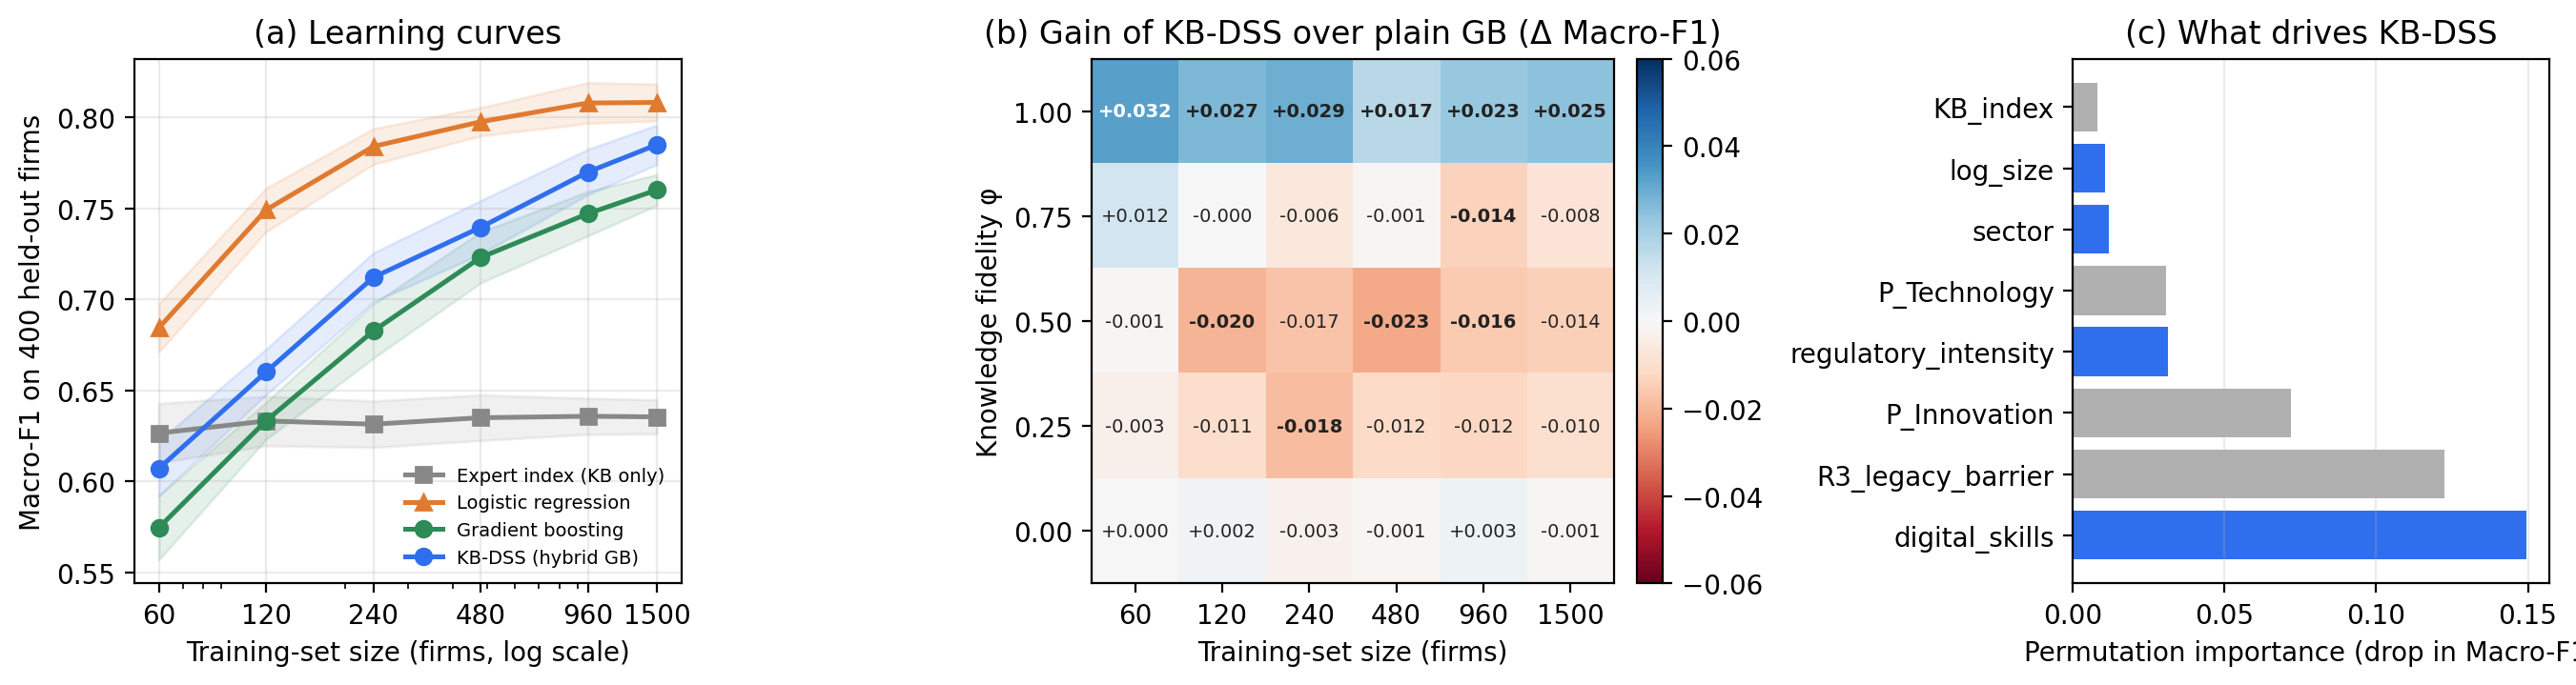
\includegraphics[width=0.98\textwidth]{figures/fig2.png}
\caption{(a)~Learning curves: mean Macro-F1 on 400 held-out firms with 95\% confidence bands over 12 stratified splits. (b)~Knowledge-fidelity map: mean gain of KB-DSS over plain gradient boosting in Macro-F1 for each fidelity level \(\varphi\) and training-set size; bold cells have a 95\% CI that excludes zero. (c)~Permutation importance of the eight most important KB-DSS features on one 400-firm hold-out; blue bars are knowledge features.}
\label{fig:results}
\end{figure*}

\subsection{What the Model Uses and How It Explains}

Permutation importance shows that KB-DSS relies mainly on the knowledge-compressed signal [Fig.~\ref{fig:results}(c)]. Shuffling the expert index lowered Macro-F1 by 0.267, against 0.020 for cloud adoption, 0.017 for sector, and 0.010 for legacy debt, the strongest raw inputs. This pattern is consistent with the learner using raw indicators to correct the expert model where it is incomplete: cloud adoption, sector, and firm size are the inputs to the cloud-by-size interaction and sector effects that no rule encodes. For one held-out firm, KB-DSS predicted Medium readiness (probability 0.834) and reported Innovation and Data as the weakest pillars. It flagged the legacy barrier (\(R_3\), activation 0.50) and analytics without a base (\(R_6\), 0.46) as negative rules, alongside data--AI synergy (\(R_1\), 0.45) as a positive one. Its recommended actions were to strengthen innovation and data first and to mitigate legacy debt with low cloud adoption. Each element of this output traces to a named pillar or rule, which a plain classifier cannot provide.

\subsection{Implications for Decision Support}

The results suggest a simple deployment rule. Below about 150 labeled firms, start from the expert index or KB-DSS. With several hundred firms, a regularized linear model is as accurate, and the knowledge layer remains useful for explanation and as insurance against noisy labels. The fidelity protocol itself is a practical tool: before deployment, a team can degrade its own rule base and check whether the measured gain behaves like the \(\varphi=1.0\) row of Fig.~\ref{fig:results}(b) or like the \(\varphi=0.0\) row.

\FloatBarrier
\section{Limitations}

The benchmark is synthetic. This makes the study transparent and exactly reproducible, but it does not show that KB-DSS predicts the readiness of real firms. Four of the six rules share their functional form with terms in the generator, so the \(\varphi=1.0\) results are an upper bound for a well-specified expert model; the fidelity protocol was introduced precisely to show how the gain falls when that assumption fails. Validation on real enterprise survey or platform data, which the script accepts through its \verb|--data| option, is the main open task.

The expert weights and rules were set by the author from maturity-model and TOE logic rather than elicited from a panel. A Delphi or AHP elicitation would make the knowledge layer more defensible and would allow the fidelity of real expert knowledge to be estimated. The fidelity operator permutes indicators, which models an expert who attends to the wrong evidence; other failure modes, such as wrong rule signs or miscalibrated weights, are not tested.

The Table~\ref{tab:models} and Table~\ref{tab:ablation} comparisons use corrected resampled tests, but the sweep intervals in Fig.~\ref{fig:results}(b) are uncorrected and therefore optimistic, as discussed in Section~IV-C. Hyperparameters were fixed and not tuned for any model, which favors no method but may understate the best attainable accuracy of each. Finally, readiness is measured at one point in time; transformation is a process, and a longitudinal formulation would require panel data.

\section{Conclusion}

This paper presented KB-DSS, a knowledge-based decision-support model that predicts digital transformation readiness from enterprise innovation data by injecting five expert pillars, six signed fuzzy rules, and an expert index into a gradient-boosting learner. Its main contribution is a knowledge-fidelity protocol that measures what expert knowledge is worth. On a reproducible benchmark, correct knowledge lifted Macro-F1 by 0.075 with 60 training firms and by 0.022 with 1500. The gain fell as knowledge fidelity fell, and fully misspecified knowledge added nothing beyond 60 firms. Knowledge also absorbed the full effect of 15\% label noise. With 1600 training firms, no corrected difference from plain boosting or logistic regression was significant. For entrepreneurs and innovation managers, who typically have few labeled cases and strong domain heuristics, the evidence supports using expert knowledge as an explicit, auditable, and testable input to AI-based readiness decisions.

\section*{Data and Code Availability}

The data are synthetic and fully reproducible. The single script \texttt{dtr.py} generates the benchmark, runs every experiment, and writes Fig.~\ref{fig:framework}, Fig.~\ref{fig:results}, Table~\ref{tab:models}, Table~\ref{tab:ablation}, and a metrics file with fixed random seeds. It is available at \url{https://github.com/Vineethsamba/kb-dss}. Running \texttt{python dtr.py} reproduces all reported numbers in about five minutes on a laptop CPU, and \verb|python dtr.py --data firms.csv| applies the same study to real data with the documented schema.

\section*{Acknowledgment}

During preparation of this manuscript, AI-assisted tools were used for code development, language drafting, editing, and formatting. The author reviewed and edited the content and takes full responsibility for the manuscript. All experimental results, tables, and figures were generated by the executable code described in the Data and Code Availability statement. The author declares no competing financial interests.

\bibliographystyle{IEEEtran}
\bibliography{references}

\begin{IEEEbiographynophoto}{Vineeth Kumar Samba}
received the B.S.\ degree in computational science from Osmania University, Hyderabad, India, in 2020, and the M.S.\ degree in computer science from Monroe University, Bronx, NY, USA, in 2024. He is currently a Senior ServiceNow Developer with SoftTechers LLC, Charlotte, NC, USA. His work concerns enterprise workflow automation, knowledge-based decision support, and informed machine learning for digital transformation readiness.
\end{IEEEbiographynophoto}

\end{document}
